\documentclass[10pt,twocolumn,letterpaper]{article}

\usepackage{cvpr}
\usepackage{times}
\usepackage{epsfig}
\usepackage{graphicx}
\usepackage{amsmath}
\usepackage{amssymb}
\usepackage{subcaption}
\DeclareMathOperator*{\argmax}{arg\,max}
\DeclareMathOperator*{\argmin}{arg\,min}

% Include other packages here, before hyperref.

% If you comment hyperref and then uncomment it, you should delete
% egpaper.aux before re-running latex.  (Or just hit 'q' on the first latex
% run, let it finish, and you should be clear).
\usepackage[breaklinks=true,bookmarks=false]{hyperref}

\cvprfinalcopy % *** Uncomment this line for the final submission

% \def\cvprPaperID{****} % *** Enter the CVPR Paper ID here
\def\httilde{\mbox{\tt\raisebox{-.5ex}{\symbol{126}}}}

% Pages are numbered in submission mode, and unnumbered in camera-ready
%\ifcvprfinal\pagestyle{empty}\fi
\setcounter{page}{1}
\begin{document}

%%%%%%%%% TITLE
\title{Generating Audio for Muted Piano-Playing Video using Deep Learning}

\author{XIA Junzhe\\
{\tt\small 20493411}\\
{\tt\small jxiaaf@connect.ust.hk}
\and
YANG Baichen\\
{\tt\small 20493198}\\
{\tt\small byangak@connect.ust.hk}
\and
HUANG Zeyu\\
{\tt\small 20493631}\\
{\tt\small zhuangbi@connect.ust.hk}
}

\maketitle

% Todo: Dataset Preprocessing, Key Splitting Comparison
%



%%%%%%%%% ABSTRACT
\begin{abstract}
   It is noticed that human playing the piano effectively generates a series of well-patterned actions, i.e. the position of hands and the keys and the depth of keys being pressed down. 
   The notes that the piano generates strongly obey to this visual pattern. 
   Hence, it becomes reasonable to recognize the visual patterns from piano-playing videos and reproduce the instrumental sounds using machine learning.
   In this project, we are going to propose a deep learning approach to effectively recognize key-press gestures and produce corresponding audios afterwards.
   
\end{abstract}

%%%%%%%%% BODY TEXT
\section{Introduction}
\label{Introduction}
   The production and consumption of digital music and video are thriving in recent years, and related researches in music and video recognition have become rather important in related fields.
   Among these fields, one important problem is how to construct mapping from videos to songs, which is possible because the visual representation is a vital aspect of musics.
   To be more specific, how to conduct the conversion from video information to symbolic notation such as music scores or Musical Instrument Digital Interface (MIDI) file.
   This problem is quite realistic for music lovers as it is hard to replay a music video without music transcription support.
   
   Our target is to generate music transcription and corresponding audio from piano-playing videos without any sound information.
   Previous works have been done towards this problem by implementing traditional computer vision methods for this task.
   However, evaluation results show that these methods are either not accurate or easy to be influenced by environmental conditions.
   So in this report, we propose a more robust solution for piano video recognition and music re-generation.

   % To specify the problem, we introduce the following notations:

   % Given a muted piano playing video $\vec{V}$ where the whole keyboard should be in the screen and each key can be seen clearly.
   % Our task is to figure out the black note set $T_i^B$ and the white note set $T_i^W$ which are played at specific frame $F_i$ extracted from $\vec{V}$ and concatenate the notes together to regenerate the piano sound for this video.
   % The note set $T$ should contain the key-pressed information as well as velocity information.
   
   To accomplish this task, we divide it into three stages.

   \textbf{1) Keyboard Extraction}
   As the keyboard's location differs in different videos, the first step is to develop a method extracting the whole keyboard from the background and conduct rectification on it. 
   The extracted keyboard will be fed into the second step.

   \textbf{2) Keypress Recognition}
   After the keyboard area is extracted, our core task is to recognize finger-key correspondence and determine whether the keys are pressed or not. 
   To finish this recognition, we need to focus on the piano keys' arrangement pattern as well as the illumination circumstance.
   However, since there are often reflections, shadows and other visual noises cast on the keyboard, it is rather difficult to develop an algorithm based on traditional computer vision method.
   Therefore, a robust algorithm is required.

   \textbf{3) Velocity Evaluation}
   The velocity information is essential in audio emotion expression. 
   With a high velocity value, the song conveys stronger feelings, and vice versa. 
   Since the velocity is a kind of dynamic information, our algorithm need to analyze several neighbor frames simutaneously in order to get the estimation.

   We have developed methods to solve these three parts and received a quite good result. 
   For the \textit{Task 1}, we've tried both traditional computer vision methods and deep learning methods, finally determined to use the \textit{SIFT} method \cite{SIFT} to achieve a better outcome.
   About the \textit{Task 2}, we trained two different neural network models for black and white key-press detection. 
   Both neural network models adopt VGG-like structure\cite{VGG} with two or three layers structure as the key size is rather small for deeper convolutional neural network to learn.
   And lastly for the \textit{Task 3}, we use the LSTM structure \cite{LSTM} and feed in neighbor frames of a video to perceive the change of the keypress as well as the velocity.

   Currently, our recognition result is quite acceptable. For the keypress recognition accuracy, i.e. the music score generation, is about \(75\%\), which is notably better than traditional computer vision methods with accuracy around \(50\%\).
   And about the velocity detection, there is also a satisfactory result as the listeners can sense some emotion which is similar as the original song conveys.
   Furthermore, to get higher robustness, we've record our own dataset in addition to adopted dataset from previous researches in order to increase diversity of environmental conditions. 
   
%------------------------------------------------------------------------
\section{Related Work}
   Previous works have been done in related area and some of them are targeting at this specific problem. In this section we will give brief introduction for them and discuss their strengths and drawbacks.

   One previous solution was proposed in Gorodnichy and Yogeswaran's paper \cite{gorodnichy2006detection} where traditional computer vision method is utilized to complete the keyboard and hand extraction as well as the gesture recognition tasks.
   Detaily, this solution divides the problem into three parts: Keyboard image detection, Hand detection and Finger detection. 
   It compute the keyboard boundary according to the assumption that white keys are surrounded by nonwhite areas, i.e. the division algorithm is based on the contrast information.
   And for the hand and finger detection, it utilized the background subtraction method and crevice-detection method.
   This solution achieved this task only with traditional computer vision methods, whose cost is lower than neural network model as the latter one needs large dataset and training.
   However, these methods required a frame where there are no hands on the keyboard because the flood fill algorithm will fail if there is a hand involving in.
   Also, since illumination conditions may differ, this traditional computer vision method doesn't perform quite well under different circumstances.

   Another solution towards this problem was proposed by Akbari et al. \cite{Akbari} 
   They proposed a system of automatically annotating piano-playing video using convolutional neural networks (CNNs) and two separate binary support vector machines (SVMs).
   Though a high accuracy has been achieved in keyboard and hand detection, this solution tackles issues according to some artificially formulated rules related to the visual nature of the piano keyboard, which is hard to prove its correctness in most cases.
   Also, since it applies CNN method in all stages of the problem, the computational cost is rather high, which is unavoidable.

%------------------------------------------------------------------------
\section{Dataset}

   In this section, we will talk about our dataset source and pre-processing.

   We adopt our dataset mainly from two sources: modified from the dataset that was been used in previous work done by Akbari \cite{Akbari}; our own record.
   Both datasets are formed by two parts: muted piano-playing videos and corresponding MIDI file, where contains all the pitch and velocity information.

\subsection{Dataset Source}
   First part of our dataset is obtained from a previous research \cite{Akbari}. It consists of piano playing videos captured in different situations which may lead to enhancement of model's strength:

   \textit{Camera Position} As variations in position may lead to keyboard detection failure, this dataset's recording position contains three posibilities: $+45,\ 0,\ -45$ degrees from vertial.

   \textit{Pianists} This dataset includes $14$ different players with different hand sizes, playing styles and skin colors, which will increase robustness of the model.

   \textit{Positive and Negative Examples} This dataset also include both positive and negative examples, where negative stands for moving the hands over the keyboard without pressing any key.
   
   In this particular part of dataset, there is $71$ recorded videos and $70540$ frams in total. And we extracted about $600000$ white keys and $400000$ black keys from it. 

   However, since the first part of our dataset doesn't include velocity information, we recorded our own dataset additionally to train the network.
   Despite of velocity information, our dataset also has the following several features:

   \textit{High Resolution} Our dataset is recorded by $1080P$ camera. The keyboard resolution increased by $70\%$ than the previous dataset. We downsize the keyboard images into \(884 \times 106\) before feeding into the model, which is still even higher than the resolution of \cite{Akbari}'s dataset without downsizing.

   \textit{Music} The first dataset only contains sequentially key-press sound track, which cannot represent real music piece. 
   In our dataset, we played and recorded several master pieces to simulate real piano-playing videos.

   In our dataset, there're $22266$ frames in total, with $14536$ black key-press and $27843$ white key-press recorded.

\subsection{Dataset Preprocessing}

\subsubsection{Conversion from/to MIDI format}

To get a trainable dataset, we firstly align the beginnings and the ends of videos and MIDI audios and sample frames out of both media files in a sampling rate of $24$ fps. Then, we generates a \(N \times 88\) label for each video file recording the status of each piano key in each frame.

The output of our method is a matrix of similar shape. The matrix undergoes a reverse process to transform into a MIDI file with the same sampling rate.

\subsubsection{Splitting keys}

To help direct the model's attention, we split the input image into 88 segments, each containing one piano key object at the center as our training target. Each white key is located by dividing a image into 52 pieces along the x-axis. Each black key is located using traditional cv algorithms. Since we have resized and skewed the images into standard \(884 \times 106\) rectangles, the splitting process yields a rather promising result. Finally, we add some ``tolerance'' by widening the cropped area by 4-6 pixels on its left and right sides to avoid excessive loss of information during the cropping. 

We also introduce a second splitting stretegy called ``bundling'', where in this mode the ``tolerance'' is enlarged to the width of the centered piano key itself. We will produce images of three keys when the centered key is our training target. This method introduces more information yet more interference.

\subsubsection{Forward/backward difference of frames}

For some training tasks (e.g. Velocity Evaluation) we also need the information of the previous frame(s) and the following frame(s). Therefore for those tasks, we also calculate the forward positive difference (i.e. the absolute value of the pixel-wise difference of the current frame and its previous frame) and the backward positive difference of each image, concatenating them to form a 9 channel input data. In our implementation, we also set it possible to acquire arbitrary degree of forward/backward positive difference in case of need.

\section{Methods}

In this section we will talk about methods tried and their pros and cons. 
As discussed in Section \ref{Introduction}, we divide this problem into three stages, keyboard detection, keypress recognition and velocity evaluation.

\subsection{Keyboard Detection}
\label{Keyboard}

Towards the keyboard detection problem, we've tried three methods. 

\subsubsection{Hough Line Detection}
Firstly, we adopted a traditional computer vision method `Hough Line Detection', which is shown in Figure \ref{fig:1}. 
% It first conduct Gaussian Blurring on the picture in order to avoid noise for edge detection. 
% Then the result will be fed into the Canny Edge Detector \cite{Canny}.
Firstly, we can obtain the edge information of the picture by conducting Gaussian Blurring and Canny Edge Detection on it.
Next, we apply Hough Line Transformation \cite{Hough} on the preprocessed picture to detect boundary lines candidates. 
And since there'll be several repeated boundary line detected, we prune those repeated lines according to their slopes and positions.
% , and from here we will get 3 to 5 boundary candidates.
Finally, we determine the exact two parallel lines that bound the keyboard by examining the black and white pixel location pattern. 
% That is, if we denote the distance between two boundary lines as $d$, then we select two lines to be boundary lines when the average pixel value in the upper \(\frac{2}{3}d\) is darker than that in the lower \(\frac{1}{3}d\).

\begin{figure}[h!]
      % \begin{subfigure}{0.23\textwidth}
      %   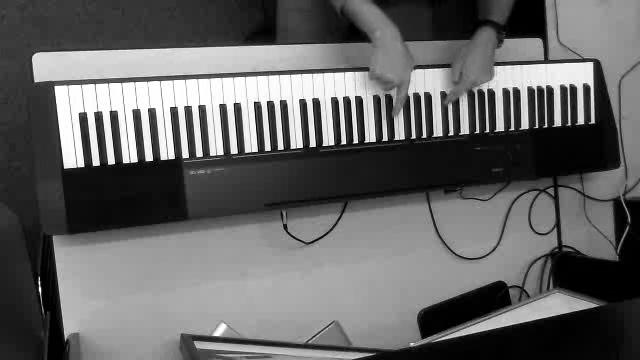
\includegraphics[width=\linewidth]{fig/1.jpg}
      %   \caption{Grayscaled Original Image} \label{fig:a}
      % \end{subfigure}\hspace*{\fill}
      \begin{subfigure}{0.23\textwidth}
        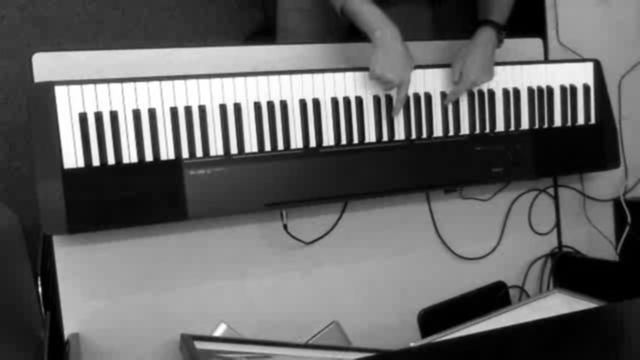
\includegraphics[width=\linewidth]{fig/3.jpg}
        \caption{Gaussian Blurred Image} \label{fig:b}
      \end{subfigure}\hspace*{\fill}
      % \medskip
      \begin{subfigure}{0.23\textwidth}
        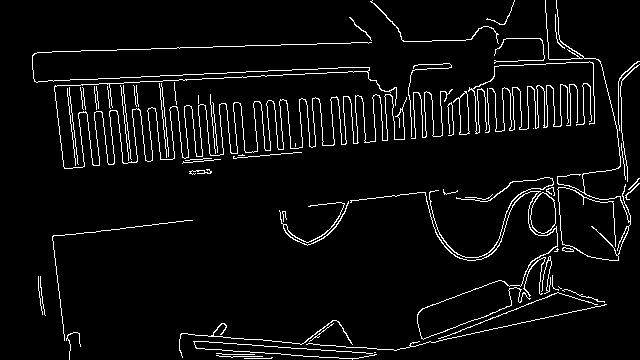
\includegraphics[width=\linewidth]{fig/4.jpg}
        \caption{Canny Edge Detection} \label{fig:c}
      \end{subfigure}
      \begin{subfigure}{0.23\textwidth}
        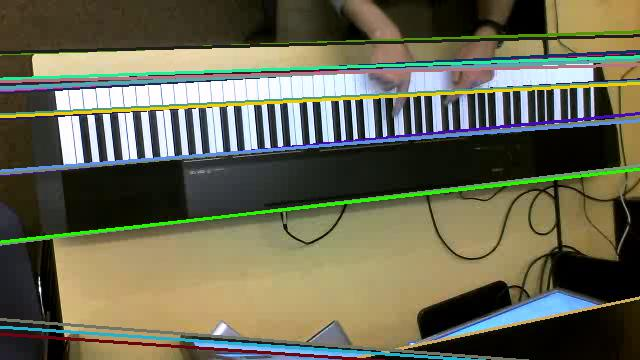
\includegraphics[width=\linewidth]{fig/5.jpg}
        \caption{Hough Line Transformation} \label{fig:d}
      \end{subfigure}\hspace*{\fill}
      % \medskip
      % \hspace{2.1cm}
      \begin{subfigure}{0.23\textwidth}
        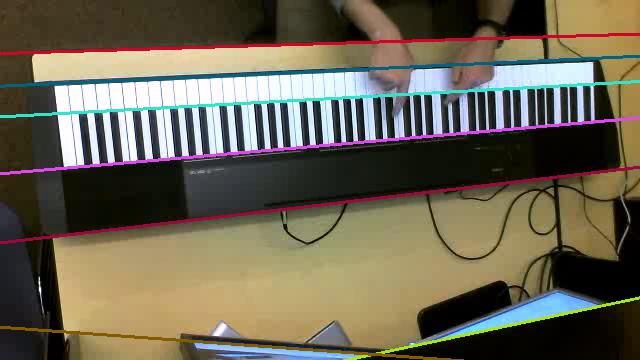
\includegraphics[width=\linewidth]{fig/6.jpg}
        \caption{Prune Repeated Lines} \label{fig:e}
      \end{subfigure}
      
      \caption{Hough Line Detection Method} \label{fig:1}
\end{figure}

However, this method has some major drawbacks. 
For one, the computational complexity of Hough Line Transformation is $O(n^3)$, where $n$ is the number of pixels. 
So the computation is quite expensive.
% Also, to achieve high accuracy, hyperparameters of Canny Edge Detector and Hough Line Transform varies a lot under different illumination circumstances.
% This leads to unstable detection performance.
In addition, to complete such detection, a frame without hand on the keyboard is needed, which is unobtainable for some videos.
Therefore, we resort to the second choice, using Deep Convolutional Neural Network.

\subsubsection{CNN Detection}

We next tried Convolutional Neural Network to detect the keyboard location. 
As the dataset doesn't offer us information about the exact location of keyboard, we manually labelled coordinates of the keyboard and feed them into a pre-trained ResNet-18 \cite{resnet} model for coordinate regression.

\begin{figure}[h!]
   \centering
   \begin{subfigure}{0.25\textwidth}
      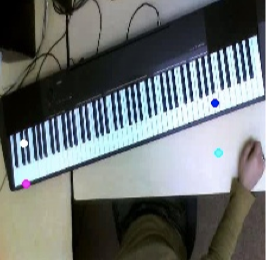
\includegraphics[width=\linewidth]{fig/8.png}
      \caption{Failure Example of CNN} \label{fig:f}
    \end{subfigure}
    \begin{subfigure}{0.30\textwidth}
      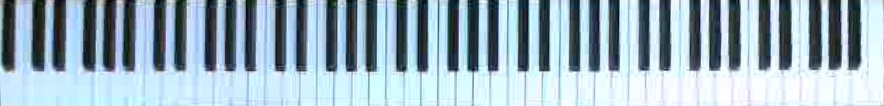
\includegraphics[width=\linewidth]{fig/9.jpg}
      \caption{SIFT Result} \label{fig:g}
    \end{subfigure}
   \caption{Comparison between CNN and SIFT} \label{fig:2}
\end{figure}

However, since the dataset is highly homogeneous because they are extracted from 71 videos, the model tends to build a mapping between image features to 71 fixed coordinate sets, which made the model’s performance on test set quite undesirable.
A failure example is shown in Figure \ref{fig:f}

We therefore turn to our third choice, the SIFT method.

\subsubsection{SIFT Detection}

Our finalized solution on this task is Scale Invariant Feature Transform (SIFT) \cite{SIFT}.

For each image in the dataset, we extract SIFT descriptors \(V_i^{1\times128}\) \((i=0,1,2,3)\) for pixel patches containing the four keyboard corners in each image using the coordinates we've labelled in the previous method.

In test time, we derive the four keyboard corners by finding the point whose SIFT descriptors are most similar to the ground truths, i.e.
$$P_i^* =\argmin_P\sum_{k=0}^{64}{\sqrt{\sum_{j=0}^{128}(V_j^P-V_{ij}^k)^2}}$$

The result shows that this method is quite robust and accurate in determining the keyboard location.
Under most circumstances, the method can extract the keyboard correctly and entirely.
A comparison example is shown in Figure \ref{fig:2}

\subsection{Keypress Recognition}

Now that we have obtained the extracted keyboard image from background, we are able to further conduct keypress recognition task on it.
In the following discussion, we will develop CNN models to conduct keypress recognition. 
Before going into different data-processing methods, we first talk about common loss function for the following networks.

\subsubsection{Loss Function}
The loss function we used is \textbf{Binary Cross Entropy Loss}, which can be described as following:
\begin{align*}
   w^*=&\argmin_w-\sum[y_i\log{w(x_i,\theta)} \\
      &+(1-y_i)\log(1-\log{w(x_i,\theta)})]+\lambda||w||_2
\end{align*}

The reason why we adopt this loss function is that we are targeting at a binary labelling problem.
That is, our dataset $D = \{(x_1, y_1), (x_2, y_2), \cdots, (x_n, y_n)\}$ where $x_n\in\mathbb{R}^{C\times H\times W}$ and $y_n\in\{0,1\}$, and data pairs are independent with each other.
After defining our loss function, our next step is to process the data and set up the network model.

\begin{figure}[h!]
   \begin{subfigure}{0.2\textwidth}
      \centering
      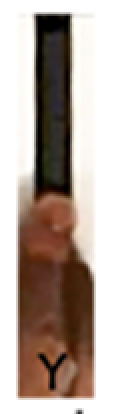
\includegraphics[width=0.33\linewidth]{fig/15.png}
      \caption{Single Key Split} \label{fig:k}
    \end{subfigure}\hspace*{\fill}
    \begin{subfigure}{0.2\textwidth}
      \centering
      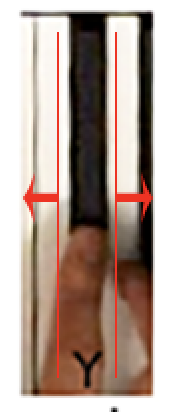
\includegraphics[width=0.5\linewidth]{fig/14.png}
      \caption{Key Bundling} \label{fig:l}
    \end{subfigure}
   \caption{Comparison between two splitting modes} \label{fig:4}
\end{figure}   

\subsubsection{Whole Keyboard Detection}
\label{Keypress-keyboard}

   Our first attempt is to put the whole keyboard and corresponding frame note label into the neural network, trying to recognize both the pressing pattern as well as key location by one network.
   We utilized a deep convolutional neural network solution for this task since it could preserve spatial information of the picture and focus its attention on some particular region.
   Our set our CNN structure to be VGG-like, the design is shown in the Figure \ref{fig:h}

   Since this method doesn't require any data preprocessing on the derived data from Task \ref{Keyboard}, it is quite easy to prepare data.
   However, it's noticed that in our train set, some keys are frequently pressed while some are pressed rarely.
   This kind of keypress inbalance leads to weakness in the detection.
   Also, as hands are comparatively small than the whole keyboard, the network tends to focus on other factors such as illumination circumstance instead of little hand movement, which lower down the recognition accuracy.

   Due to the above drawbacks, the network's recognition accuracy is not quite good. Therefore we tried the idea of splitting all the keys and recognize them respectively.

   \begin{figure}[h!]
      \centering
      \begin{subfigure}{0.4\textwidth}
         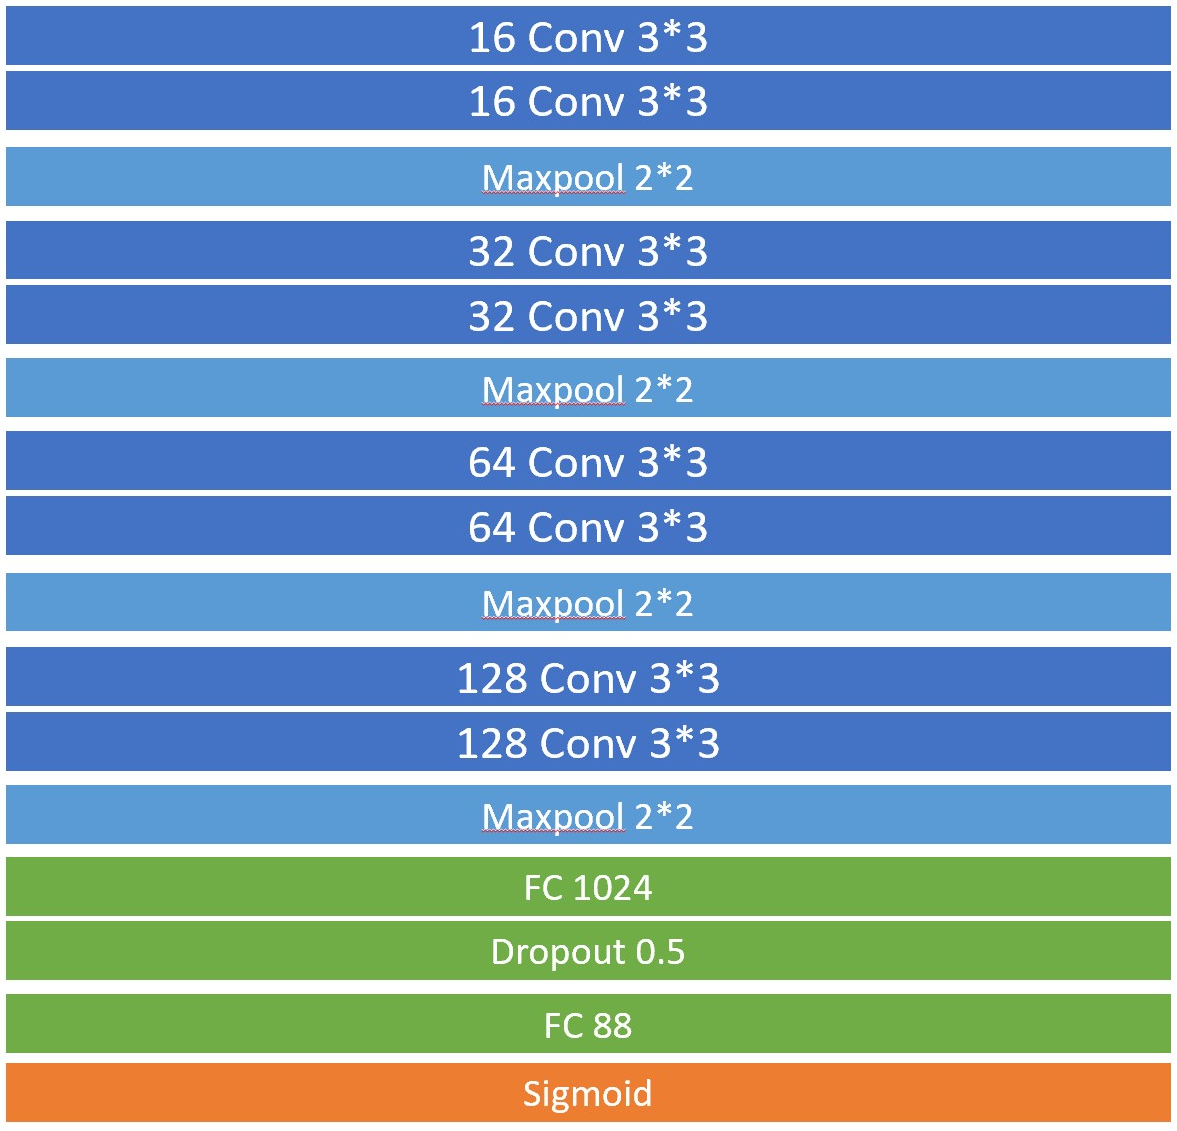
\includegraphics[width=\linewidth]{fig/10.png}
         \caption{CNN for Whole Keyboard Detection} \label{fig:h}
       \end{subfigure}
       \begin{subfigure}{0.4\textwidth}
         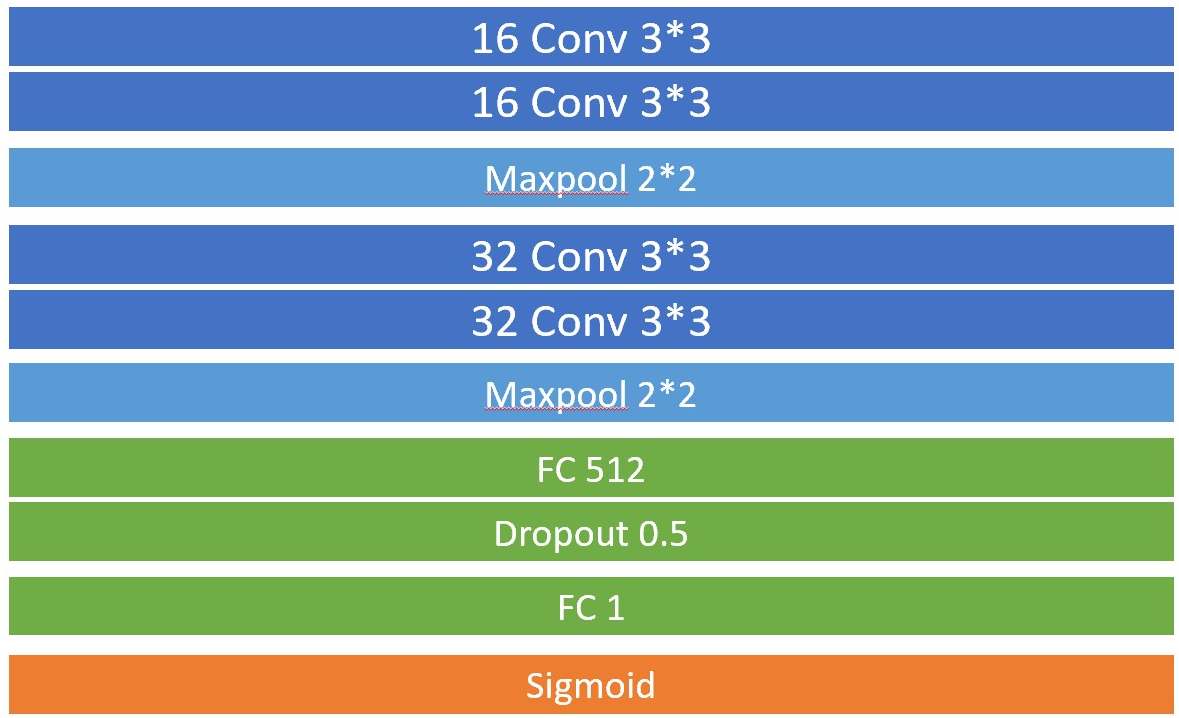
\includegraphics[width=\linewidth]{fig/11.png}
         \caption{CNN for Key Splitting} \label{fig:i}
       \end{subfigure}
       \begin{subfigure}{0.4\textwidth}
         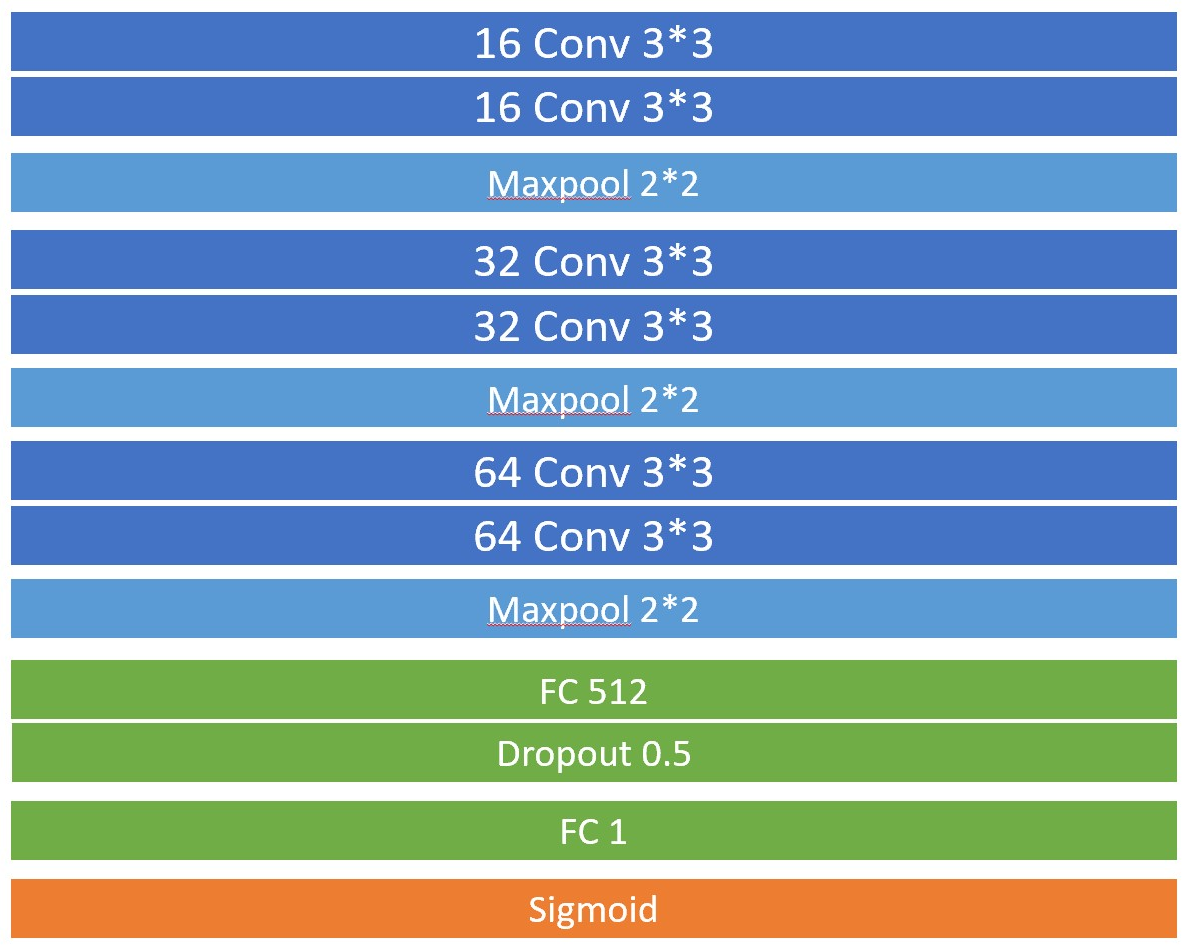
\includegraphics[width=\linewidth]{fig/12.png}
         \caption{CNN for Key Bundling} \label{fig:j}
       \end{subfigure}
      \caption{CNN structures for Keypress Recognition} \label{fig:3}
   \end{figure}

\subsubsection{Single Key Splitting}

   Our next attempt is to split the keyboard into keys and train a neural network to identify whether the specific key is pressed or not. 
   Since the input dimension and information contained are less than the previous one, we constructed a neural network which has fewer layers than the whole keyboard detection model.
   The model structure is shown in Figure \ref{fig:i}

   This model works quite well on our dataset, and achieves higher accuracy than the previous mehthod as data partition becomes finer.
   And the inbalance problem mentioned in Section \ref{Keypress-keyboard} won't affect the recognition any longer.

   However, we noticed that the single key extraction may lose some information on key-pressing as neighbor keys can become comparison to the selected key.
   Also, hand gesture could be shown more clearly with neighbor keys included.
   Therefore, to achieve better accuracy, we consider to bundle nearby keys and feed it into the neural network.

\subsubsection{Key Bundling}

   Lastly, we bundle neighbor keys together to construct a new dataset. 
   Since bundling too many keys tends to incur more noise, we determined the bundling number $B = 3$, including left-1 and right-1. (See Figure \ref{fig:4})
   However, this is a hyperparameter and will be tuned during the experiment.
   And as the image size becoming larger, we added two CONV layers and generated a new architecture, which is shown in Figure \ref{fig:j}.

   Comparing to the second method, it includes extra information about neighbor keys and hand motion surrounded without introducing the inbalance problem mentioned in Section \ref{Keypress-keyboard}.
   With respect to the experiment result, its accuracy indeed becomes higher and even exceeds best current result.

\subsection{Velocity Evaluation}

   Last part of our task is to evaluate the velocity of each keypress. 
   In MIDI file, the velocity is recorded as an integer value ranges from $0$ to $127$. 
   So our objective is to detect motion in neighbor frames and make a prediction on the velocity value of that key press.
   
   Since the prediction is related to several consecutive frames which requires sequence learning technique, we therefore choose the LSTM structure for this task. (See Figure \ref{fig:5}) 

   \begin{figure}[h!]
      \centering
      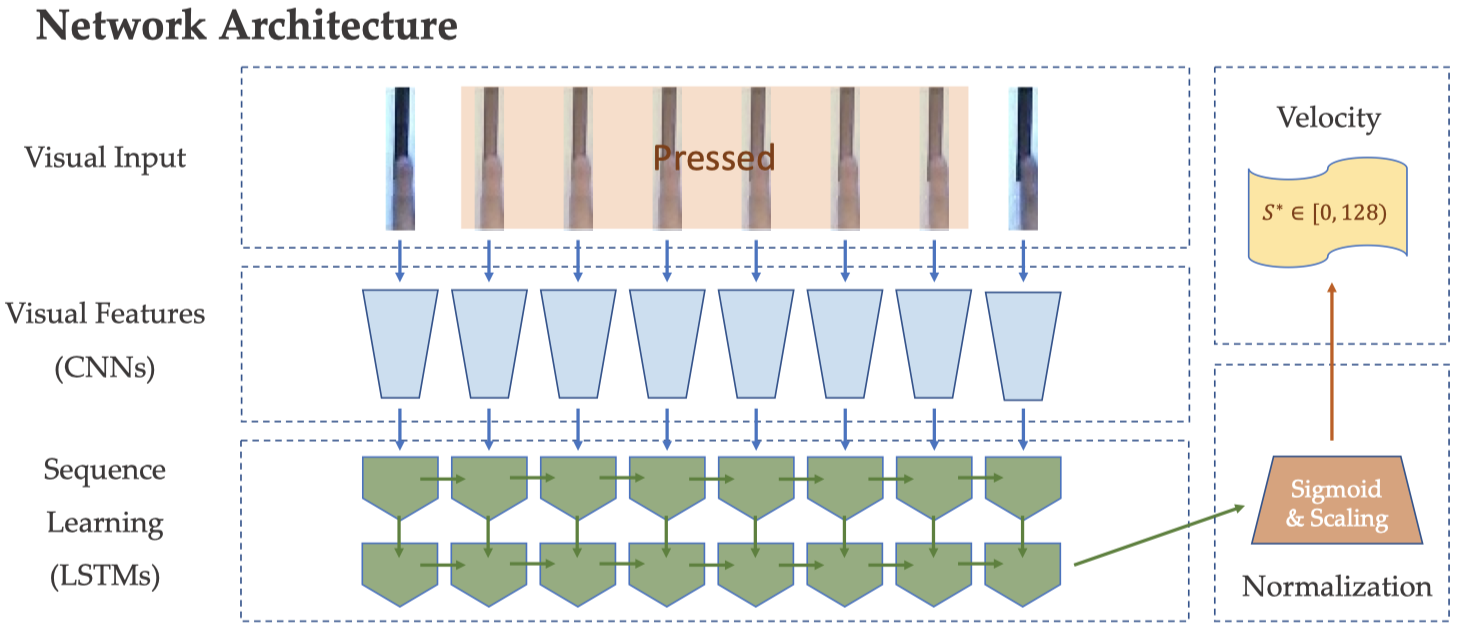
\includegraphics[width=\linewidth]{fig/13.png}
      \caption{LSTM Architecture for Velocity Evaluation} \label{fig:5}
   \end{figure}

\section{Experiments}

In this section we will talk about our experiment settings and current results.

\subsection{Metrics}

\subsection{Results}

Two criterion: precision and recall

Minimum Edit Distance


\subsection{Results}

Accuracy

Demo Video

\section{Conclusion and Future Work}

{\small
\bibliographystyle{ieee}
\bibliography{egbib}
}

\end{document}
